%=======================================================================
\chapter{Getting Started}
\label{ch:getting-started}
%=======================================================================

\tuprolog{} can be enjoyed from different perspectives:
\begin{enumerate}
  \item as a \textit{Prolog user}, you can exploit its Integrated Development
        Environment (IDE) and Graphical User Interface (GUI) to consult, edit, and run Prolog programs, as you would do with any other Prolog system---and you can do so in any of the supported platforms (Java, .NET, Android, Eclipse).
  \item as a \textit{Java user}, you can include \tuprolog{} in any Java project,
        thus bringing the power of Artificial Intelligence to the Java world; the \tuprolog{} API provides many classes and methods for exchanging data
        between the Java and the Prolog worlds.
        Though you can do so using your preferred IDE, the \tuprolog{} plugin
        for the Eclipse platform is probably the most practical choice for this purpose, as the \tuprolog{} perspective provides all the views over the Prolog world in an Eclipse-compliant, effective way.
  \item as a \textit{.NET user}, analogously, you can add \tuprolog{} to any
        Visual Studio project (including the related IKVM libraries, as detailed in Chapter \ref{ch:mpp-in-dotnet}, or just manually compile your .NET application with the necessary DLL files in the build path. The \tuprolog{} API, which is nearly identical to the Java one, provides for proper data exchange
        between the .NET and the Prolog worlds.
  \item finally, as an \textit{Android user}, you can both enjoy the \tuprolog{} app
        to consult, edit, and run Prolog programs, as you would do with any other Prolog system, and --perhaps more interestingly-- exploit the \tuprolog{} Java API for developing Android applications, adding intelligence to your next Android app.
\end{enumerate}

%=======================================================================
\section{\tuprolog{} for the Prolog User}
\label{sec:prolog-user-perspective}
%=======================================================================

As a Prolog user/programmer, you might want to start running your existing programs.
%
There are three ways to do so:
\begin{itemize}
  \item by using the graphical \tuprolog{} GUI (both in Java and .NET)
  \item by using the console-based \tuprolog{} CUI  (Java only)
  \item by using the \texttt{Agent} class to execute a Prolog program in a `batch' form---that is, running the program provided as a text file (Java only).
\end{itemize}

The first two forms are rather obvious: after starting the GUI/CUI, you will get a rather standard graphical/character-based Prolog user interface (Figure \ref{fig:tuprologGUICUI}).

The GUI includes an editing pane with syntax highlighting, a toolbar providing facilities to load/save/create theories, load/unload libraries, and show/hide the the debug information window; at the bottom, the status bar provides information, as detailed below.

The GUI can be launched either by double-clicking the \tuprolog{} executable (\texttt{2p.jar} in Java, \texttt{2p.exe} in .NET), or by manually issuing the commands

\texttt{java -cp \emph{dir}/2p.jar alice.tuprologx.ide.GUILauncher}

\noindent or

\texttt{2p.exe}

\noindent in .NET, respectively.

Analogously, the command-line CUIconsole (available in Java only) can be launched by issuing the command:

\texttt{java -cp \emph{dir}/2p.jar alice.tuprologx.ide.CUIConsole}

\noindent The CUIconsole can be quitted issuing the standard \texttt{halt.} command.


\begin{figure}
  \includegraphics[width=300px]{images/tuprologIDE.png}\\
  \includegraphics[width=300px]{images/tuprologCUI.png}\\
  \caption{The standard \tuprolog{} GUI and CUI.}\label{fig:tuprologGUICUI}
\end{figure}

The third form, available in Java only, is basically an auxiliary tool to batch-execute a Prolog program: it takes the name of a text file containing a Prolog theory as its first (mandatory) argument and optionally the goal to be solved as its second argument, then starts a new Prolog virtual machine, performs the demonstration, and ends.
%
The \texttt{Agent} tool is invoked from the command line as follows:

\texttt{java -cp \textit{dir}/2p.jar alice.tuprolog.Agent \textit{theoryfile}
\{\textit{goal}\}}

\noindent For instance, if the file \verb|hello.pl| contains the mini-theory:

\texttt{go :- write('hello, world!'), nl.}

\noindent the following command causes its execution:

\texttt{java -cp \textit{dir}/2p.jar alice.tuprolog.Agent hello.pl go.}

\noindent resulting in the string \texttt{hello, world!} being printed on the standard output.

\noindent Alternatively, the goal to be proven can be embedded in the Prolog source by means of the \texttt{solve} directive, as follows (Figure \ref{fig:tuprologAgent}):

\texttt{:- solve(go).}\\
\indent\texttt{go :- write('hello, world!'), nl.}

\noindent Quite obviously, in this case no second argument is required.

\begin{figure}
  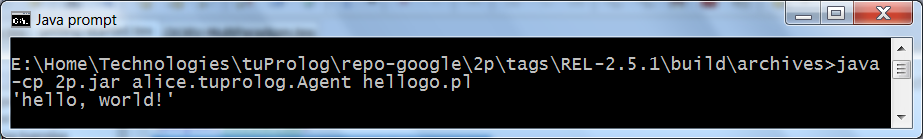
\includegraphics[width=300px]{images/tuprologAgent.png}
  \caption{The \tuprolog{} Agent tool.}\label{fig:tuprologAgent}
\end{figure}

%------------------------------------------------------
\subsection{Editing theories}
\label{sec:editing-theories}
%------------------------------------------------------

The editing area allows multiple theories to be created and modified at the same time, by allocating a tab with a new text area for each theory.
%
The text area provides syntax highlighting for comments, string and list literals, and predefined predicates.
%
Undo and Redo actions are supported through the usual \keycap{Ctrl}+\keycap{Z} and \keycap{Ctrl}+\keycap{Shift}+\keycap{Z} key bindings.

\begin{figure}
\centering
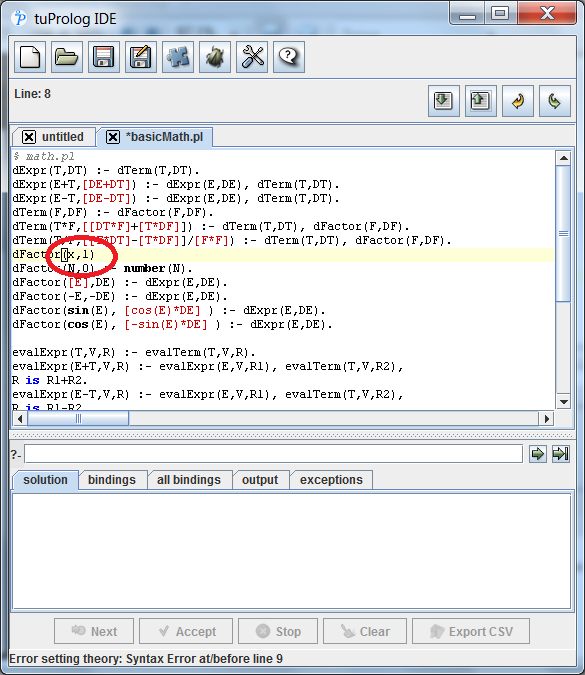
\includegraphics[width=7cm]{images/syntaxErrorFound}
\caption{Syntax error found when setting a theory}
\label{fig:syntax-error-found}
\end{figure}

\begin{figure}
\centering
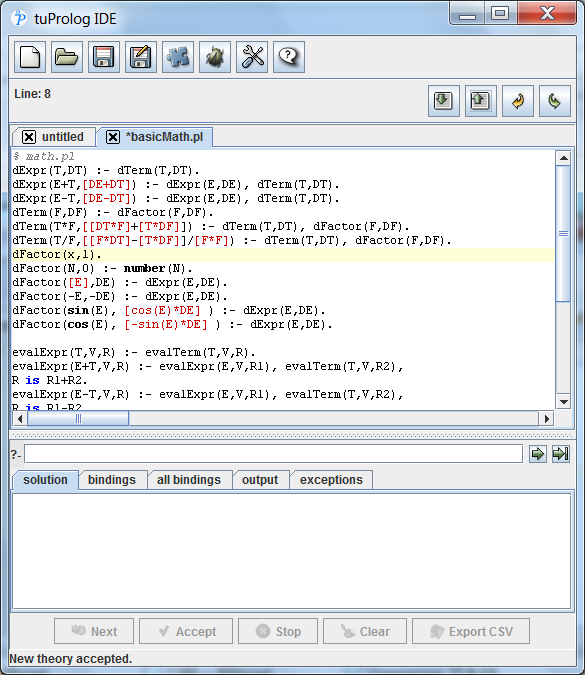
\includegraphics[width=7cm]{images/setTheorySucceeded}
\caption{Set theory operation succeeded}
\label{fig:set-theory-succeeded}
\end{figure}

The toolbar contains four buttons: two are used to upload/download a theory to/from the Prolog engine, two support the classical Undo/Redo actions.
%
Explicit uploading/downloading of theories to/from the Prolog engine is a consequence of \tuprolog{}'s choice to maintain a clear separation between the engine and the currently-viewed theories: in this way,
\begin{itemize}
  \item theories can be edited without affecting the engine content: they can also be in an inconsistent state, since syntax checking is performed only upon loading;
  \item changes in the current database performed by the Prolog program via the \texttt{assert}/\texttt{retract} do not affect the theory shown in the editor, which maintains the original user theory.
\end{itemize}
%
Accordingly, the \textit{set theory} button uploads the text in the editor window to the engine, while the \textit{get theory} button downloads the current engine theory (possibly changed by the program) from the engine to a new editor tab.

However, for the user convenience, a logical shortcut is provided that automatically uploads the current theory to the engine whenever a new query is issued: obviously, if the theory is invalid, the query will not be executed.
%
Manual uploading is still needed whenever the theory in the editor window is modified via other other means than the built-in editor---for instance, after a \predicate{consult/1} goal, or via other editors.

The status bar at the bottom of the window reports information such as the cursor line number or syntax errors when setting an invalid theory.
%
For instance, Figure \ref{fig:syntax-error-found} shows the error message due to a missing dot at line 8, while Figure \ref{fig:set-theory-succeeded} shows the status message after the error has been corrected, and the theory successfully uploaded.

%------------------------------------------------------
\subsection{Solving goals}
\label{sec:solving-goals}
%------------------------------------------------------

The console at the bottom of the window contains the \textit{query textfield} and a multi-purpose, tabbed information panel.

The \textit{query textfield} is where to write and execute queries: the leftmost (\guibutton{Solve}) button triggers the engine to find the first (and then the subsequent) solution(s) interactively, while the rightmost (\guibutton{Solve All}) button forces the engine to find all the solutions at once.
%
Pressing the \keycap{Enter} key in the textfield has the same effect as pressing the \guibutton{Solve} button.

\begin{figure}
\centering
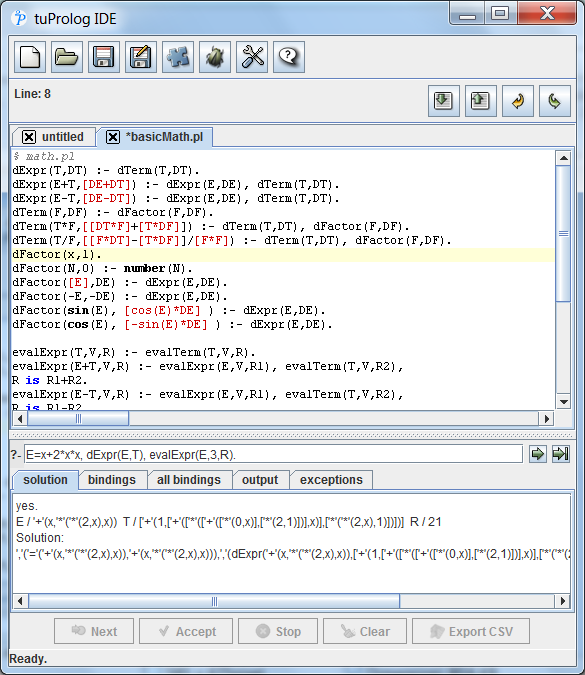
\includegraphics[width=7cm]{images/gui-solutions}
\caption{The solutions tab showing the query solution.}
\label{fig:gui-solutions}
\end{figure}

\begin{figure}
\centering
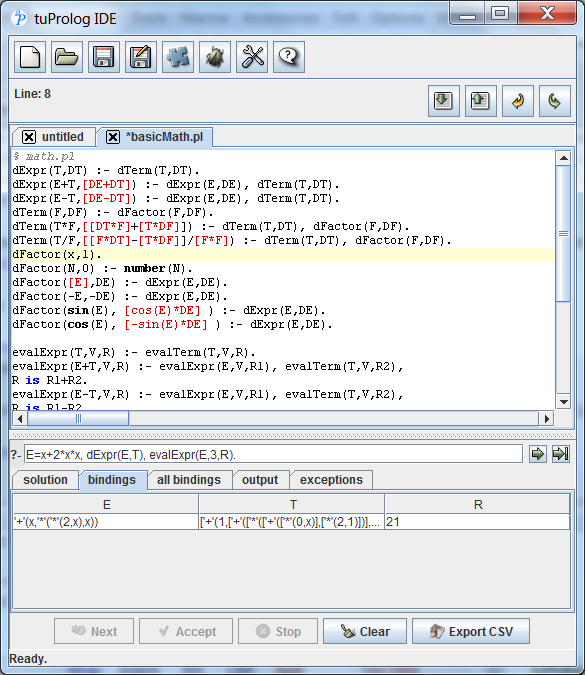
\includegraphics[width=7cm]{images/gui-bindings}
\caption{The bindings tab showing the bindings of query solution.}
\label{fig:gui-bindings}
\end{figure}

The subsequent area below contains five panes:
%
\begin{itemize}
\item the \textit{solution pane} shows the query solutions (see Figure \ref{fig:gui-solutions}): proper control buttons are provided to iterate
    through multiple solutions;

\item the \textit{binding} and the \textit{all bindings} panes show the variable bindings in tabular form, for a single solution or for all solutions, respectively (see Figure \ref{fig:gui-bindings}); here, too, proper control buttons are provided to clear the bindings pane and export the tabular data in a convenient CSV format;

\item the \textit{output pane} shows the output performed by the program via \texttt{write} and other console I/O predicates (Figure \ref{fig:gui-output}).
    Please note that output performed by Java methods -- that is, methods invoked on Java objects via \classname{JavaLibrary} -- are \textit{not} captured and displayed in this view: for further information on this topic, refer to Section \ref{sec:java-library}.
    %
    Again, control buttons are provided to clear the output pane.

\item the \textit{exceptions} pane shows the exceptions raised during the query demonstration: if exceptions are triggered, it gains focus automatically and is color-highlighted for the user convenience (Figure \ref{fig:gui-exceptions}).
\end{itemize}

\begin{figure}
\centering
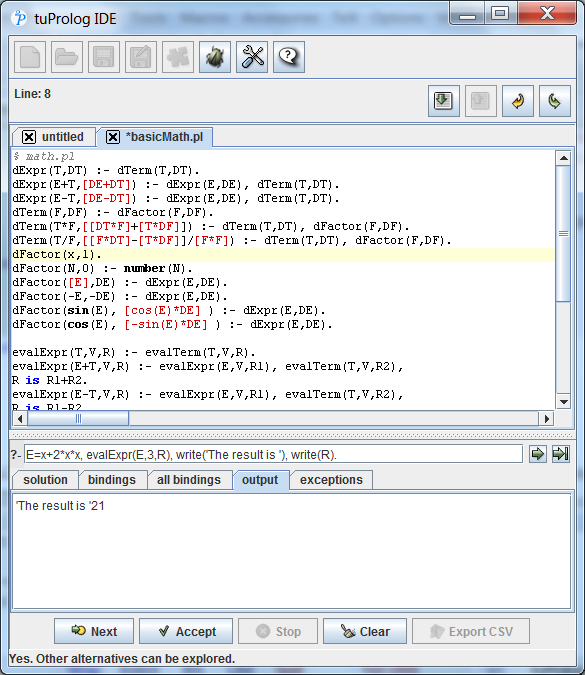
\includegraphics[width=7cm]{images/gui-output}
\caption{The output tab showing the query printing.}
\label{fig:gui-output}
\end{figure}

\begin{figure}
\centering
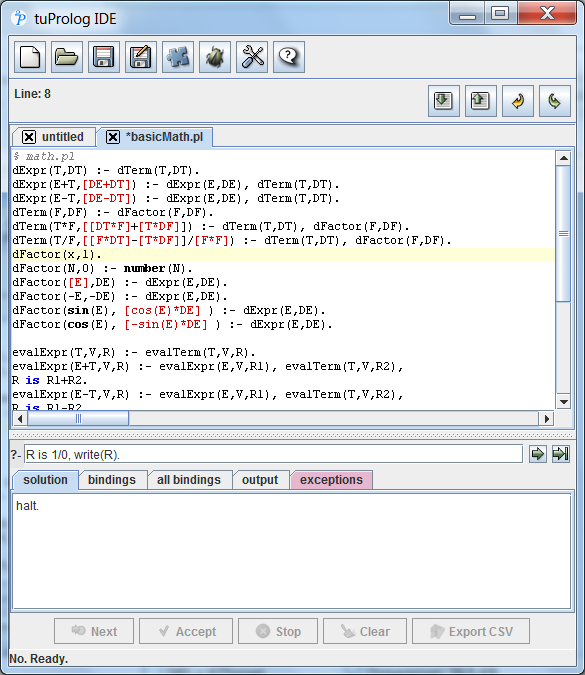
\includegraphics[width=7cm]{images/gui-exceptions}
\caption{The exceptions tab gaining focus and showing raised exceptions.}
\label{fig:gui-exceptions}
\end{figure}
Query and answers are stored in chronological order, and can be explored by means of \keycap{Up} and \keycap{Down} arrow keys from the query input textfield.

The \guibutton{Stop} button makes it possible to stop the engine if a computation takes too long or a bug in the theory is causing an infinite loop. 
%(Note: like most Prolog systems, \tuprolog{} does not normally perform \textit{occur check}, for performance reasons; this check can be enabled via the proper built-in predicate---see Section \ref{sec:basic-library} for details.)

With respect to this issue, it is worth noting that, unlike most Prolog systems, \tuprolog{} performs the so-called \textit{occur check} systematically: so, \texttt{unify\_with\_occurs\_check/2} and \texttt{=/2} behave identically (see Section \ref{sec:basic-library}).

%------------------------------------------------------
\subsection{Debugging support}
\label{ssec:debugging-support}
%------------------------------------------------------

Debug support in \tuprolog{} is actually limited compared to other professional Prolog systems: however, \textit{warnings} and \textit{spy information} are available.

To this end, the \guibutton{View Debug Information} button opens the Debug window which lists \textit{i)} all the warnings, produced by events such as the attempt of redefining a library predicate, and \textit{ii)} the step-by-step spy information of the engine computation during a goal demonstration.

Warnings are always active, while spy notification has to be explicitly enabled (and disabled) via the built-in \predicate{spy/0} (\predicate{nospy/0}) predicate.
%
Figure \ref{fig:gui-debug} shows an example of spy information for a goal: by default, information is presented in a collapsed form, but single nodes (or all the nodes) can be expanded using the toolbar buttons, to access more detailed information.

\begin{figure}
\centering
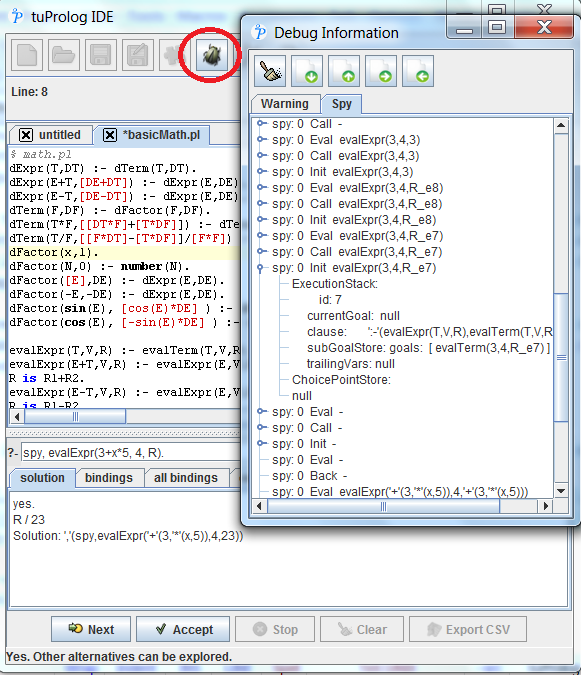
\includegraphics[width=7cm]{images/gui-debug}
\caption{Debug Information View after the execution of a goal.}
\label{fig:gui-debug}
\end{figure}

%------------------------------------------------------
\subsection{Dynamic library management}
\label{ssec:dynamic-library-management}
%------------------------------------------------------

As anticipated above, \tuprolog{} engines are dynamically extensible via \textit{libraries}: each library can provide its own set of new built-in
predicates and functors, as well as a related theory.
%
By default, the standard set of libraries is loaded into any newly-created engine, but the library set of each engine can be easily modified via the \textit{Library Manager}, which is displayed by pressing the \guibutton{Open Library Manager} button in the toolbar (Figure \ref{fig:gui-library-manager}).

\begin{figure}
\centering
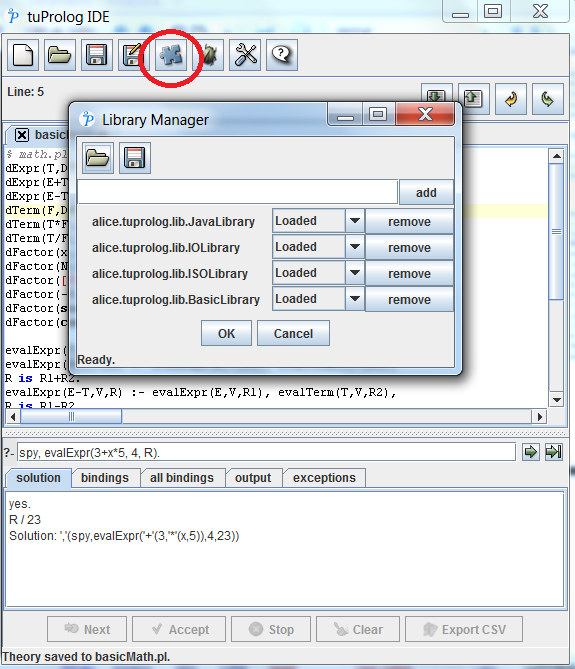
\includegraphics[width=7cm]{images/gui-library-manager}
\caption{The Library Manager window.}
\label{fig:gui-library-manager}
\end{figure}

This dialog displays the list of the currently loaded libraries---by default,
\classname{BasicLibrary}, \classname{IOLibrary}, \classname{ISOLibrary}, \classname{JavaLibrary}.
%
Other libraries can be added by providing the fully qualified name of the
library class in the textfield, and pressing the \guibutton{Add} button: the added library will be displayed with an initial \textit{Unloaded} status.
%
Please note that any further class needed by a library must be in the system classpath, or the library will not be added to the manager/loaded into the engine.

The library manager takes into account the effects of the \verb|load_library/1| and \verb|unload_library/1| predicates/directives, too: so, for instance, after a goal such as \verb|load_library('TestLibrary'), test(X).|, a new entry for \verb|TestLibrary| would be displayed.

If the addition of a library to the manager or its loading into the engine fails (for instance, due to an invalid class name, or a class not extending the
\classname{alice.tuprolog.Library} class, etc.), an error message will be displayed
in the status bar.

Finally, the \guibutton{config} button opens the configuration dialog (Figure \ref{fig:gui-configuration}), which provides access to a set of options and tunings.

\begin{figure}
\centering
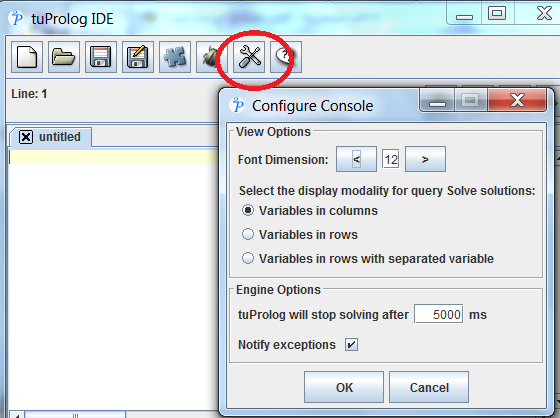
\includegraphics[width=7cm]{images/gui-config}
\caption{The configuration window.}
\label{fig:gui-configuration}
\end{figure}

%=======================================================================
\section{\tuprolog{} for the Java Developer}
\label{sec:java-user-perspective}
%=======================================================================

As anticipated above, the Java developer can include \tuprolog{} in any of his projects, exploiting the \tuprolog{} API to access the Prolog engine(s) from his Java program..
%
The easiest way to do so it to exploit the Java plugin available for the Eclipse IDE, which adds a specific \textit{tuprolog perspective} specifically suited for the needs of the Java/Prolog user (Figure \ref{fig:tuprologPluginGUI}).

\begin{figure}
  \includegraphics[width=300px]{images/tuprologPluginGUI.png}
  \caption{The \tuprolog{} plugin GUI for Eclipse.}\label{fig:tuprologPluginGUI}
\end{figure}

This perspective is mainly designed to support the development of multi-language, multi-paradigm applications (see Chapters \ref{ch:mpp-in-java}, \ref{ch:mpp-in-dotnet}), but can also be used as a standard Prolog console, writing (or loading) the Prolog theory in the editor and writing the query in the proper textfield---although the direct use of the \tuprolog{} GUI is probably faster for this purpose.

To use \tuprolog{} in Eclipse, one first needs to create a new \tuprolog{} project, and add a new theory file (\texttt{*.pl}) to the project.
%
To this end:%, three procedures are possible:
\begin{itemize}
  \item either select \texttt{New $>$ Project} from the Package Explorer's context menu, then select the \texttt{tuProlog} item;
  \item or, select \texttt{File $>$ New $>$ Other $>$ tuProlog $>$ tuProlog Project} from the main menu;
  \item or, press the \textit{New tuProlog Project} buttons in the \tuprolog{} toolbar (Figure \ref{fig:plugin1}.
\end{itemize}

In any case, a dialog appears (Figure \ref{fig:plugin2}) which prompts for the project name (default: \texttt{My\_Prolog\_Project}) and the desired Prolog libraries (the default set is proposed).

\begin{figure}
  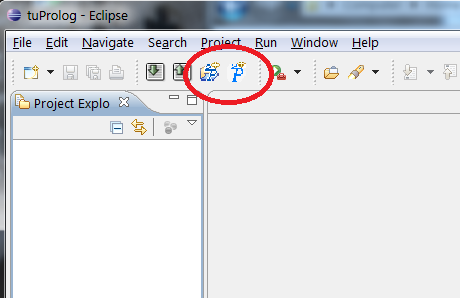
\includegraphics[width=200px]{images/plugin1.png}
  \caption{The \tuprolog{} toolbar}\label{fig:plugin1}
\end{figure}

\begin{figure}
  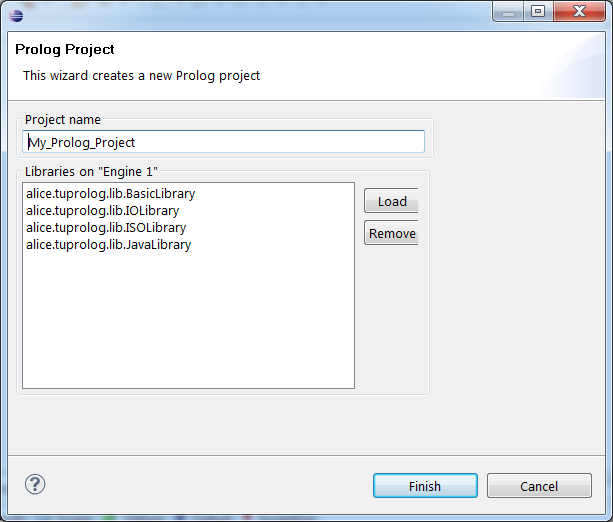
\includegraphics[width=200px]{images/plugin2.png}
  \caption{new \tuprolog{} project}\label{fig:plugin2}
\end{figure}

\begin{figure}
  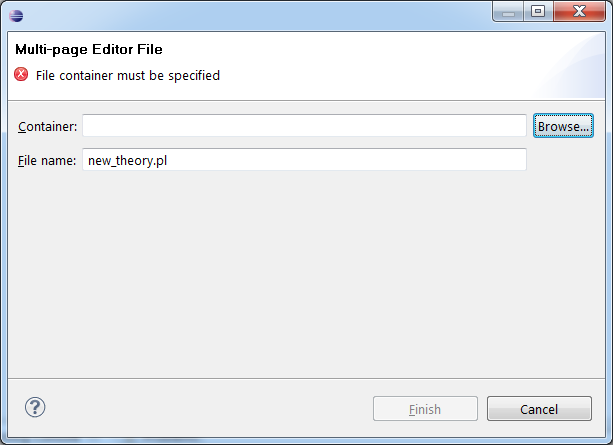
\includegraphics[width=200px]{images/plugin3.png}
  \caption{new \tuprolog{} file}\label{fig:plugin3}
\end{figure}

\begin{figure}
  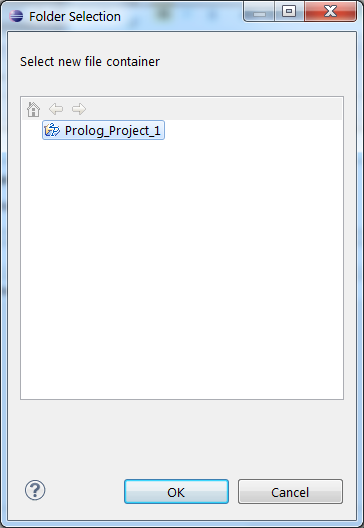
\includegraphics[width=200px]{images/plugin4.png}
  \caption{new \tuprolog{} file $>$ Browse...}\label{fig:plugin4}
\end{figure}

\begin{figure}
  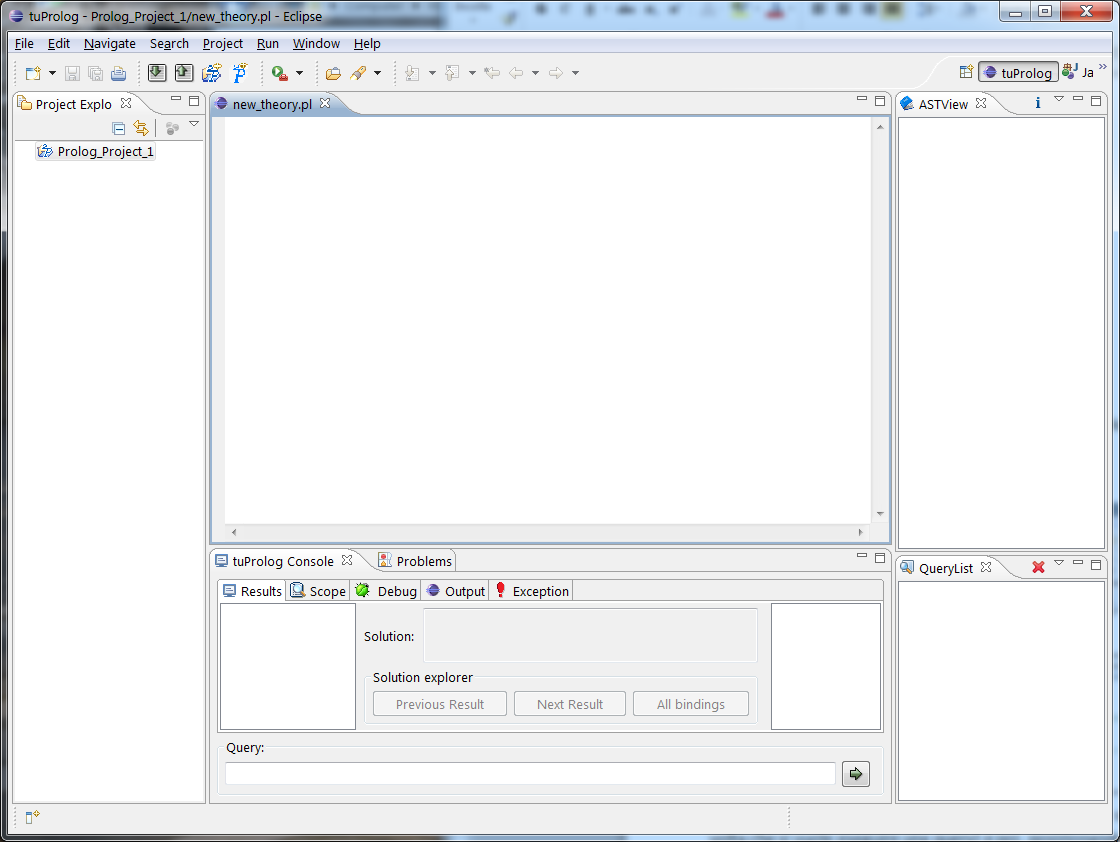
\includegraphics[width=200px]{images/plugin5.png}
  \caption{the \tuprolog{} perspective}\label{fig:plugin5}
\end{figure}

\begin{figure}
  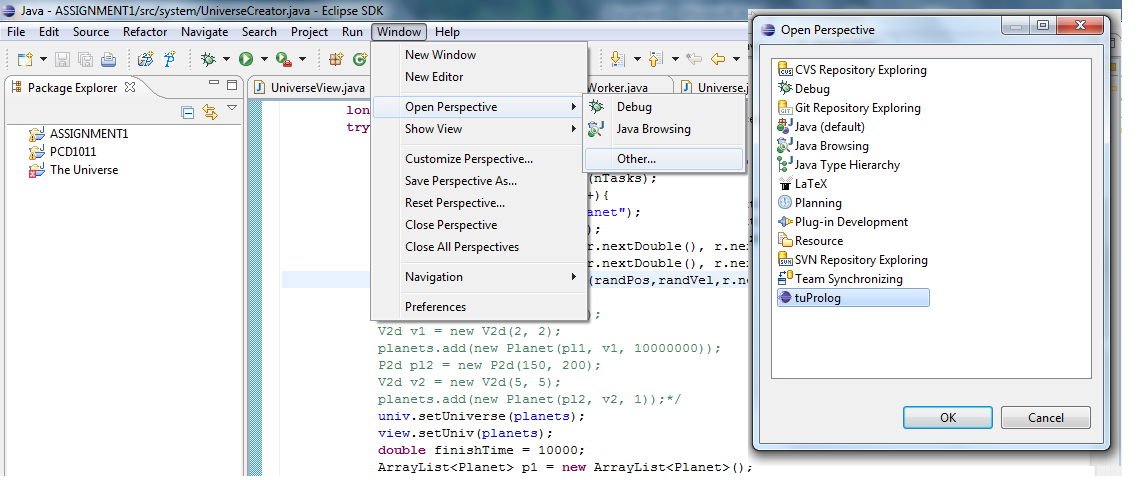
\includegraphics[width=200px]{images/plugin6.png}
  \caption{opening the \tuprolog{} perspective}\label{fig:plugin6}
\end{figure}

Pressing the \textit{New tuProlog File} button, a dialog appears which asks for the theory name (default: \texttt{new\_theory.pl}) and the file container, i.e. the tuProlog project where the new file has to be added (Figure \ref{fig:plugin3}); this is a mandatory argument. Pressing the \textit{Browse..} button, a new dialog proposes the current \tuprolog{} projects (Figure \ref{fig:plugin4}); again, the same result can be achieved via menu selection  (\texttt{File $>$ New $>$ Other $>$ tuProlog $>$ tuProlog Theory}). After confirming, the \tuprolog{} perspective automatically opens (Figure \ref{fig:plugin5}). Again, the same result can be achieved via the \texttt{Window $>$ Open Perspective} menu (Figure \ref{fig:plugin6}).

Once the theory has been written (or loaded), the theory file must be saved, either clicking the save icon in the toolbar, or choosing the \texttt{File $>$ Save} option, or hitting CTRL+S on the keyboard; this is mandatory before issuing any query.
The query can be written in the bottom console, and is executed either by pressing the Enter key, or by clicking the \textit{Solve} button.


\begin{figure}
  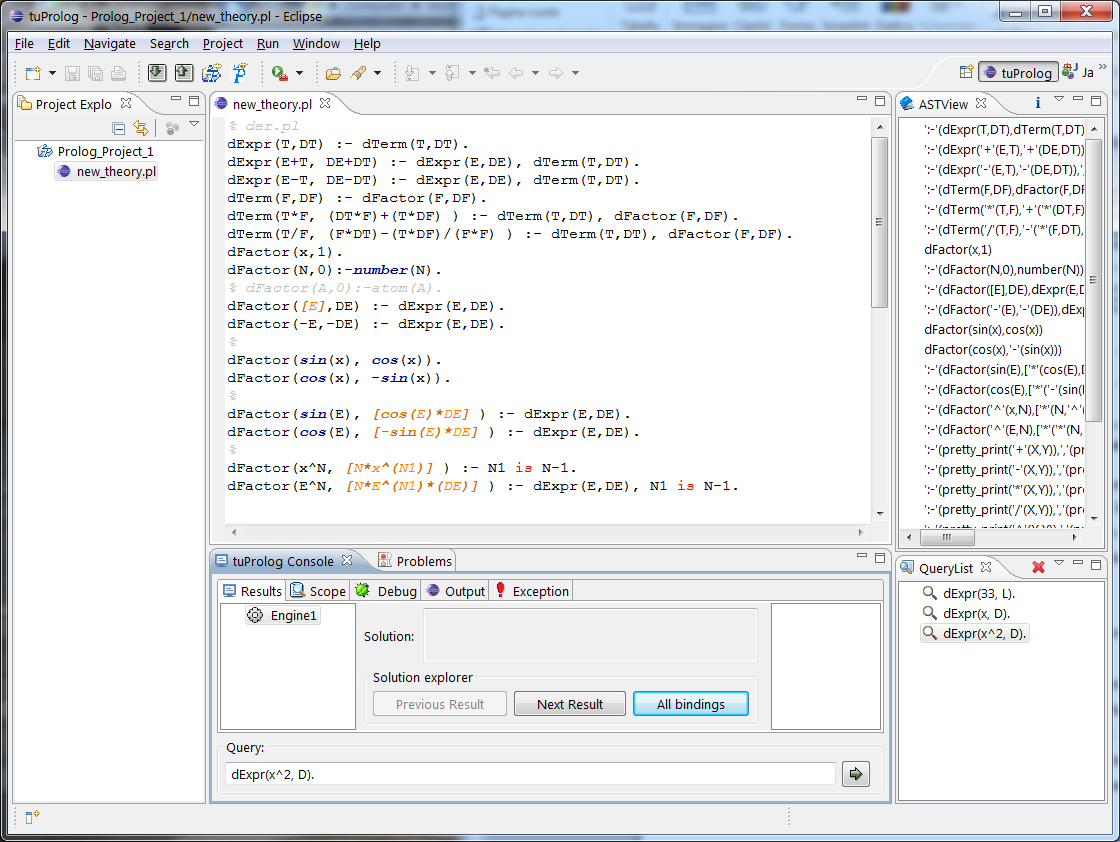
\includegraphics[width=4cm]{images/plugin7.png}
  \caption{executing queries, available views}\label{fig:plugin7}
\end{figure}

\begin{figure}
  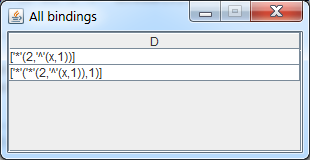
\includegraphics[width=200px]{images/plugin8.png}
  \caption{all variable bindings}\label{fig:plugin8}
\end{figure}

\begin{figure}
  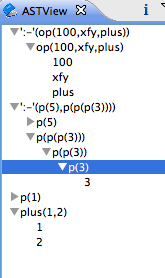
\includegraphics[width=200px]{images/plugin9.png}
  \caption{AST view (expanded)}\label{fig:plugin9}
\end{figure}

\begin{figure}
  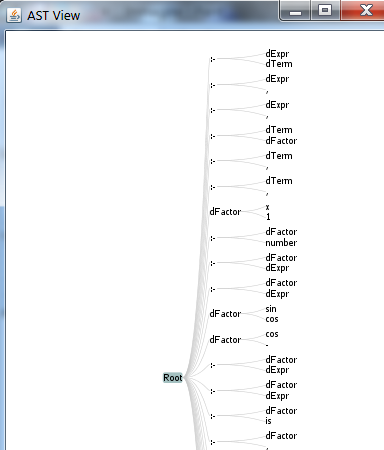
\includegraphics[width=200px]{images/plugin10.png}
  \caption{AST view (big term, expanded)}\label{fig:plugin10}
\end{figure}

The query results are shown in different views (Figure \ref{fig:plugin7}):
\begin{itemize}
  \item the \tuprolog{} Console view reports the query results: the variable bindings are also available pressing the \textit{All bindings} button (Figure \ref{fig:plugin8}).
  \item the Output view shows the program output messages;
  \item the QueryList view on the left side reports the list of all he executed queries, which can then be re-selected and re-executed in a click;
  \item the AST view shows the (dynamic) set of current clauses: pressing the \texttt{i} icon, a graphical view of the Abstract Syntax Tree produced by the Prolog parser is shown (Figures \ref{fig:plugin9} and \ref{fig:plugin10}).
\end{itemize}

It is worth highlighting that multiple \tuprolog{}  engines can be handled simultaneously: each engine can be selectively loaded with each own set of libraries and theories, and can be separately queried.
%
Moreover, in case of undeclared terms, a direct warning is issued in the plugin editor  (Figure \ref{fig:plugin11}).

\begin{figure}
  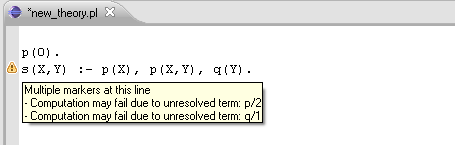
\includegraphics[width=200px]{images/plugin11.png}
  \caption{warning for undeclared terms}\label{fig:plugin11}
\end{figure}

%=======================================================================
\section{\tuprolog{} for the .NET Developer}
\label{sec:dotnet-user-perspective}
%=======================================================================

Since \tuprolog{}.NET is the result of an automatic conversion of the Java bytecode via IKVM \cite{ikvm}, everything in the Prolog user experience is identical whether the .NET or the Java GUI is used (see Section \ref{sec:prolog-user-perspective} above).

The .NET developer, however, can exploit \tuprolog{} in a .NET project, accessing its API from a program written in potentially any language available in the .NET platform.
%
Since no plugin is available for the de-facto standard tool used by most .NET programmers (i.e., Microsoft Visual Studio), there is no immediate way to see \tuprolog{} at work from within Visual Studio; however, the \tuprolog{} libraries can be easily added as external references for exploiting the available APIs, as one would do with any other library or third-party software.

For specific information about multi-paradigm programming in the context of the .NET platform, please refer to Chapter \ref{ch:mpp-in-dotnet}.


%=======================================================================
\section{\tuprolog{} for the Android User}
\label{sec:android-user-perspective}
%=======================================================================

Since \tuprolog{} is written in Java, the Java-Android developer wishing to include \tuprolog{} in an Android project can proceed very similarly to the Java developer, adding \texttt{tuprolog.jar} to the project libraries---though no plugin is available for this platform.

The Prolog-Android user, instead, can take advantage of the \tuprolog{} app, which shares the same core and libraries as the standard Java version, the only difference being the redesigned GUI--with special regard to the interaction with the file system.

Upon the application loading, the splash screen appears, immediately followed in a few seconds by the \textit{Home Activity} (Figure \ref{fig:android12}, left).
%
At the top, the name of the selected theory is reported (none at the beginning); below is the query textfield.
%
Four buttons enable the user to execute a query, ask for the next solution (when applicable), show the current solution and view the output console.
%
The menu button triggers the pop-up shown in Figure \ref{fig:android12} (right), whose main feature is \textit{List Theories}.

\begin{figure}
  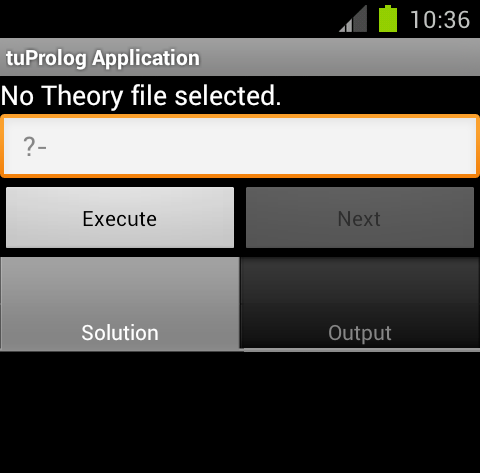
\includegraphics[width=200px]{images/android1.png}
  
\includegraphics[width=200px]{images/android2.png}
  \caption{Home Activity (left) and its pop-up menu (right).}\label{fig:android12}
\end{figure}

Indeed, in \tuprolog{} for Android theories are not loaded directly in the Prolog engine from the file system, as in the standard Java version: rather, following Android recommendations, a \textit{theory database} mediator is provided, so as to separate the loading of a theory from its validity check---the latter being performed only when the theory is actually selected for being loaded into the engine. In this way, invalid theories (possibly incomplete, work-in-progress theories) can seamlessly be stored in the theory database, independently of their invalid nature.

So, theories of interest must be first loaded into the theory database (Figure \ref{fig:android34}, left): then, the theory to be actually loaded will be selected from such theories.
%
More precisely, to add a theory to the database, the menu option \textit{Import Theory to Database} is provided (Figure \ref{fig:android34}, right): a new activity opens that lets you browser the device's file system (Figure \ref{fig:android56}, left). Only the files that can be actually selected for addition to the theory database are shown: after a theory is successfully imported, the activity remembers the path for the next time, so as to make it faster to import multiple files.

\begin{figure}
  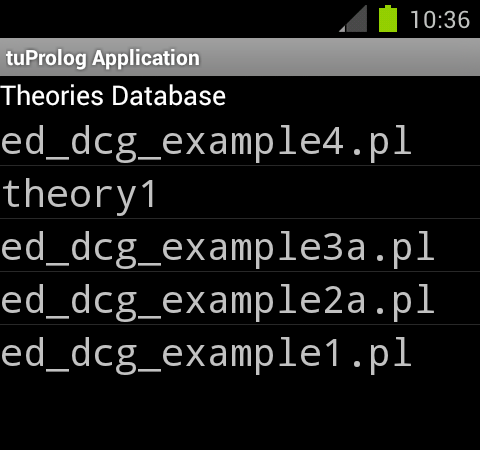
\includegraphics[width=200px]{images/android3.png}
  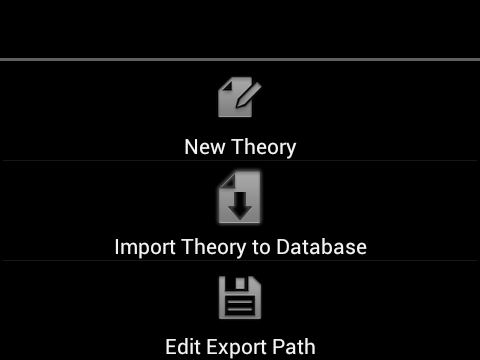
\includegraphics[width=200px]{images/android4.png}
  \caption{Theory database (left) and context menu (right)}\label{fig:android34}
\end{figure}

\begin{figure}
  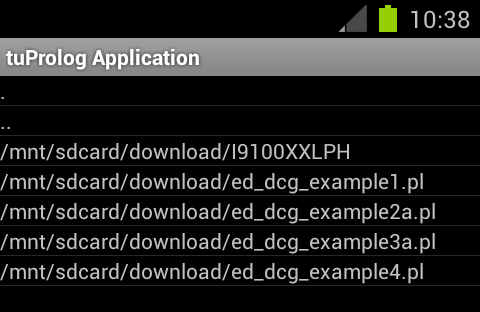
\includegraphics[width=200px]{images/android6.png}
  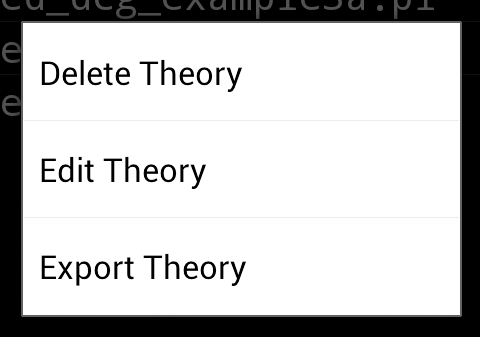
\includegraphics[width=200px]{images/android5.png}
  \caption{Browsing theories (left) and theory operations (right)}\label{fig:android56}
\end{figure}

\begin{figure}
  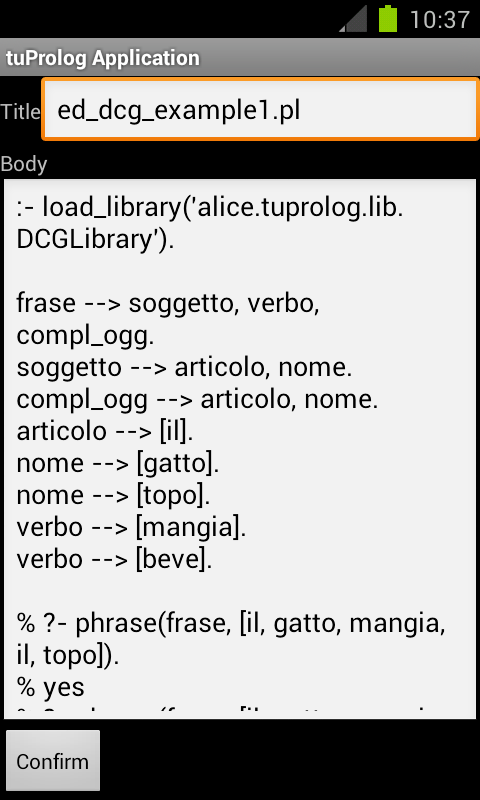
\includegraphics[width=200px]{images/android7.png}
  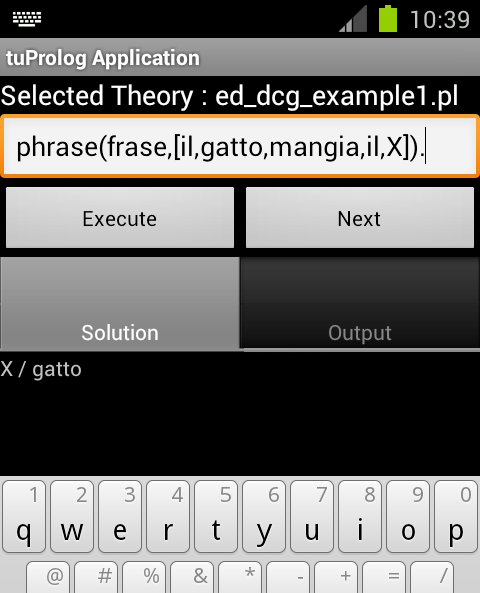
\includegraphics[width=200px]{images/android8.png}
  \caption{Theory editing (left) and query execution (right)}\label{fig:android78}
\end{figure}

Theories in the database can be deleted, edited and exported in a (long-)click, using the proper the context menu item (Figure \ref{fig:android56}, right). The export path can be changed via the \textit{Edit Export Path} in the activity menu.

Editing (Figure \ref{fig:android78}, left) applies both to existing (loaded) files and to brand new theories: to create a new theory, just click on \textit{New Theory} option in the context menu.
%
After editing, to make your changes permanent, the modified theory must be saved to the theory database by clicking the \textit{Confirm} button: alternatively, the back button discards changes.

When a valid theory is loaded, a query can be written in the input field (Figure \ref{fig:android78}, right): an auto-complete mechanism is available which exploits the previous queries to speed up the typing process.
%
Pressing \textit{Execute}, the query solution is shown in the \textit{Solution} tab, along with variable bindings; any output performed by the application is available in the \textit{Output} tab. If multiple solutions exist, the \textit{Next} button is enabled and can be exploited to browse them---the corresponding output being shown in the \textit{Output} tab.
